% g-2 Introduction
\chapter {Introduction}
In particle physics, \gmtwo of the muon, and \gmtwo in general, is an important and deep probe into the Standard Model (SM). The gyromagnetic ratio, $g$, represents the coupling strength of a particle to the type of helicity flipping transitions mediated by magnetic fields, and the $\hbox{--}2$ portion denotes the subtraction of the expected value of the gyromagnetic ratio, leaving only the anomalous magnetic moment, $a$.  The quantity acts as both a seed for new particle physics models and a scythe on proposed models.   Contributions to the quantity depend on the gamut of fundamental interactions and constants of the universe in the SM: quantum electrodynamics (QED), Weak and Strong interactions all playing important roles.  Precision measurement of \gmtwo facilitates development of standard model extensions of somewhat analogous interactions of particles inspired by SM particles.
\todo{expand this a bit, too terse}

\subsection{Magnetic Moment Fundamentals}

A thorough understanding of muon \gmtwo begins with classical model for a magnetic moment.  An entity attains a magnetic moment when the object has net correlation between electric charge and angular momentum.  Equation \ref{} shows how such a correlation can be calculated.  The angular momentum can be physical, $\vec{L}$, or intrinsic spin, $\vec{S}$, so the equation holds, classically at least, for volumes and point-like particles with spin. The caveat is that there is an proportional constant g-factor that must be included in the spin calculation of the equation giving rise to equation \ref{eqn:spin-magnetic-moment} for magnetic moments that arise due to spin.

\begin{equation}
\label{eqn:magnetic-moment-integral}
\todo{insert integral equation for magnetic moment} 
\end{equation}

\begin{equation}
\label{eqn:spin-magnetic-moment}
\vec{\mu} = g \frac{e}{2m}\vec{S}
\end{equation}

The g-factor can vary extensively between different particles.  The proton and neutron for instance \note{look up values and get refernce}.  For point-like particles the g-factor was calculated to be exactly 2 by Dirac \todo{get reference}.  Initial experiments measuring electron and muon \gmtwo were consistent with the calculation that $g\equiv2$.  Discrepancies did not begin to arise for several years, but that is discussed in \ref{sec:history-expt} rather than here.  The short of it is that interactions with the quantum vacuum shift the value of $g$ at the \SI{0.1}{\percent} level.

Intuitively, a magnetic moment is similar to macro-scale magnet that all children are all familiar with.  One of the important behaviors exhibitited is a tendency to anti-align with external magnetic fields.  Such macro behavior is useful in compasses to align with the Earth's magnetic North Pole and seen with bar magnets where oppositive ends attract.  The behavior holds true in the micro as well, and this behavior turns out to be crucial in pulsed nuclear magnetic resonance (pNMR) measurements.  Precession is another important behavior arising from a non-zero magnetic moment.  A magnetic field orthogonal to the particle's magnetic moment causes the magnetic moment vector to rotate in plane orthogonal as prescribed by equation \ref{eqn:classical-precession}.

\begin{equation}
\label{eqn:classical-precession}
\omega = \frac{\mu B}{2 m}
\end{equation}

\section{Motivation}

There are two major questions that need answers to motivate the muon \gmtwo experiment.  The first is: "Why measure the anomalous magnetic moment?", and the second is: "Why use muons?".  

To the first charge, there are many appropriate replies.  One answer is that it is a simple measurement in principle.  The experimenters need a polarized volume of particles, an external vertical magnetic field, and a technique to determine the spin direction. Another, more phenomological answer is that it serves as a multi-faceted probe into quantum field theories in general and the Standard Model in particular.  Calculating the value for \gmtwo requires consideration of effects arising in Quantum Electrodynamics (QED), Electro-Weak (EW) Theory, and Quantum Chromodynamics (QCD).  It traversing nearly the entire space of the Standard Model.

And, to the second question, there are physics considerations and practical considerations.  The physics consideration weighs in with the desire for sensitivity to the intricacies of the Standard Model.  The more intricate, higher order interactions general come into the playing field with mass suppression, $\propto (\frac{m}{M})^2$, or possibly to a higher power.  The relative mass ratio between the electron and the muon enhance these terms by a factor of $(\frac{105.66}{0.511})^2 \approx 42,750$ \note{add reference}!  The previous argument begs the question though, "Why not use the $\tau$?".  The answer is a practical consideration; the capricious $\tau$ has a lifetime of only \SI{0.29}{\femto\second} compared to \SI{2.2}{\micro\second} for the $\mu$.  While the $\tau$ particle is appealing if a significant enough Lorenz boost could be achieve, an experiment using $\tau$ particles is simply not practical with current technology.

\subsection{Statistical Tension}

The muon \gmtwo has been measured many times over the years.  And, throughout it has been a constant probe of the Standard Model and beyond.  The experiment value has come along from a modest start when it agreed with the classical calculation of $g\equiv2$ to gradually highlighting a \SI{3}{\sigma} deviation from Standard Model predictions.  The experiments are discussed further in section \ref{sec:history-expt}.  Theoretical calculations 

\todo{I need to take notes and make a diagram here for theory and experiment values.}

\subsection{Beyond Standard Model}

Let's start the discussion with a general argument for the size of the corrections

\todo{decide which models to talk about}

\section{History of Experiment} \label{sec:history-expt}

For many years the value of both $g_e$ and $g_\mu$ were thought to be exactly $2$ as predicted for pure Dirac particles\cite{the-muon-g-2}. And, initial experiments supported the prediction that $g = 2$ \todo{cite initial expt}. That notion, however, had to be reconciled with experiment as measurement precision progressed and statistical tensions arose with the values predicted by theory.  Deviations from a pure Dirac particle were first observed in hyperfine splitting measurements of several different nuclei.  The measured deviations were not statistically significant until Kusch and Foley measured the atomic spectra of several nuclei in 1947 \cite{kusch-foley}.  The theory community quickly resolved the discrepancy with a now standard QED calculation of the lowest order self-interaction for leptons emitting and reabsorbing photons, see figure \ref{fig:schwinger-diagram}.  The Schwinger term, coined after Julian Schwinger, brought experiment and theory back into good agreement.  It served as an early triumph of QED. 

\begin{figure}
\centering
\todo{Add diagram of schwinger term}
\label{fig:schwinger-diagram}
\caption{The Feynman diagram for the so-called Schwinger term.}
\end{figure}

\subsection{Parity Violation}
The first direct measurement of the anomalous magnetic moment, \gmtwo, came later, and the muon \gmtwo much later.  The first measurement of $g_e$ happened in 1953 by H. R. Crane, et al. \todo{can't find pdf of paper}.  Subsequent theoretical calculations and supporting experimental measurements established $g_e$ as the most precisely predicted and measured quantity of QED.  As for measuring $g_\mu$, no one knew how to properly control the polarization of the muons, that is until parity violation of the Weak interaction came to light.  With parity violation baked into the Weak interactions, researchers quickly realized that pion would decay into muons polarized along the beam direction.  

\subsection{CERN-I}
Building off the Weak parity revelation, researchers measured $g_\mu$ for the first time.  In 1960 Columbia personnel measured the quantity to $5\%$, and not long after a more precise measurement came out of CERN and eclipsed it.  The experiment worked by injecting relatively low energy (83 MeV) muons into a long, narrow magnetic trap where the polarized muons would undergo both cyclotron motion and lateral drift. At the opposite end of the magnet, the muons were ejected, tagged for storage time, and stopped where the momentum direction of electron was recorded as recorded as either forward or backward.  Using this technique CERN scientists were able to achieve a precision of $0.4\%$, absolutely phenomenal for the time \cite{cern-i}.  A deviation of $1.6\,\sigma$ was present at the achieved precision.

\begin{figure}
\centering
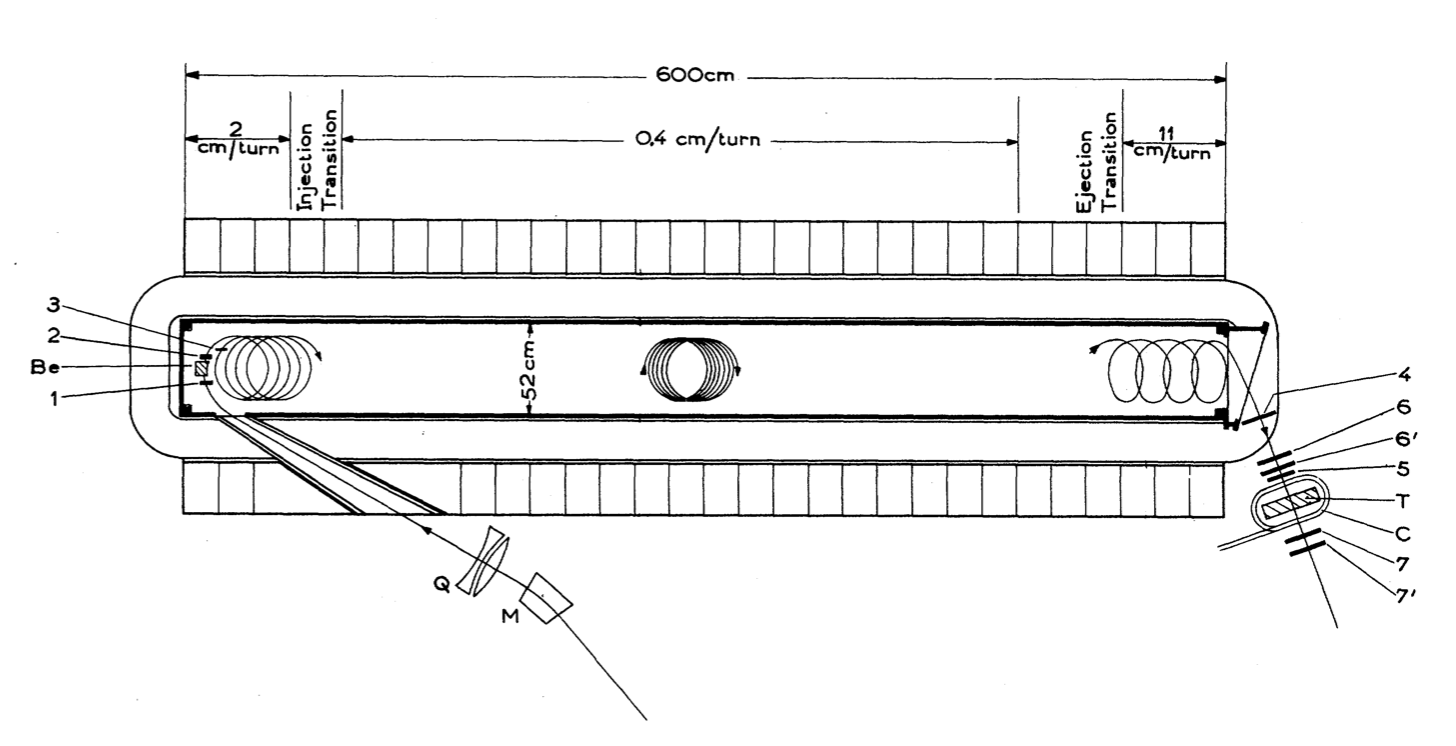
\includegraphics[width=0.9\linewidth]{fig/cern-i-diagram.png}
\label{fig:cern-i-diagram}
\caption{A diagram of the experimental setup in the first muon \gmtwo experiment at CERN. The muons enter from the lower left, go through the energy moderator to put the cyclotron radius at 19cm, drift and circles toward the ejection side of the magnetic, escape from the the magnet, stop in the fiducial block, and decay into an electron with momentum correlated to the spin direction.}
\end{figure}

\subsection{CERN-II}
The second iteration of muon \gmtwo at CERN improved vastly over the first.  CERN-II was the first muon \gmtwo to use the now familiar storage ring \cite{47y-muon-g-2}.  In order to store muons, the experiment injected a beam of protons which hit a pion production target.  A slice of the pion production phase space matched the momentum acceptance of the ring well enough to remain for several revolutions. And, some fraction of the muons produced from pion decay were mostly forward decays that lost a bit of energy and matched the ring's momentum acceptance.  The decay electrons curled inward to electron counting detectors at a rate modulated at \gmtwo frequency.  The injected muons had a relativistic $\gamma$ of 12 which allowed the researchers to measure muon spin precession for more than 130 $\mu s$ which led to determination of $a_\mu$ to \ppm{270}.

\subsection{CERN-III}
The final CERN muon \gmtwo experiment ran from 1969 to 1976.  One major innovation introduced in CERN-III was use of the so-called "magic" momentum. Observe eqn \ref{eqn:full-omega-a}, the equation for spin precession in electromagnetic fields for a relativistic muon.

\begin{equation}
\omega^\prime_a = \omega_a[1 + (1 - 1 / a \beta^2 \gamma^2)(\beta E_r / B)]
\label{eqn:full-omega-a}
\end{equation}

A muon beam at a very specific momentum, \gev{3.094}, cancels the effects of of radial electric fields which allows electrostatic focusing to be used on the muon beam instead of magnetic gradient focusing.  Another major innovation for the third CERN experiment was the use of pion injection instead of proton injection.  The measurement techniques of CERN-III were similar to CERN-II.  With the achieved improvements, the CERN team was able to drive down the uncertainty on $a_\mu$ to \ppm{7}, nearly a 40-fold improvement!

\subsection{E821 at BNL}
The most precise Muon \gmtwo experiment to date, took place at Brookhaven National Laboratory (BNL). The experiment, E821, as it was labeled for high energy physics ledgers pushed precision muon phyiscs to a new level.  E821 needed 400-fold statistics increase over it's predecessor.  In order to accommodate the necessesited higher rates, the decay electron measurement platform was separated into 24 individual calorimeters.  Another critical improvement in the experiment, E821 injected muons rather than pions, or protons.  Muon injection provided a cleaner data earlier in each fill.  The experiment design also focused on improving the homogeneity of the magnetic storage field.  The aperture of the storage region was increased to facilitate a more uniform field across the muon storage volume.  Field measurement was also improved by implementing both a suite of fixed probes always monitoring magnetic field drift outside of the storage region and a trolley outfitted with an array of 17 probes to measure the field in the storage volume periodically.  In the end, the experiment nearly achieved the initial goal of 350 ppb uncertainty on $a_\mu$, actually reaching 540 ppb uncertainty.

The E821 \gmtwo result placed the value at odds with theoretical calculations.  Depending on the theoretical models, the measurement was somewhere around $3.3\sigma - 3.6\sigma$ away from theoretical prediction, a statistical tension.  The tension remained in subsequent years, inspiring a new iteration of the muon \gmtwo experiment at Fermi National Accelerator Laboratory (FNAL). The experiment, E989, reuses the storage ring, superconducting coils, and various components from the BNL experiment.  The goal of E989 is an overall uncertainty of 140 ppb, pushing the tension to a $5\sigma$ discrepancy. Additionally, a sister experiment is being undertaken at J-PARC as a completely independent measurement of muon \gmtwo with similar sensitivity as the BNL experiment.  In a parallel effort, theoretical particle physics researchers have been pushing the precision of calculations to match pace with experiment.

\section{Theory Contributions}

The theoretical contributions to muon \gmtwo come from all corners of particle physics.  The typical diagonalization of the contributions breaks them into QED, Weak, and Strong. The relative sizes of the contributions are displayed in figure \ref{fig:sm-contributions}. The Electro-Weak contributions are well modeled, and theoretical progress involves calculating increasingly intricate Feynman diagrams.  The Strong contributions are trickier and represent a larger challenge to the theory community.  The theory community as set a similar precision goal as the E989 collaboration, \SI{140}{ppb}, following a similar time frame, around 2020.

\todo{discuss main difference between electron and muon then focus only on muon}

\begin{figure}
\includegraphics[width=0.9\linewidth]{fig/SM-contributions.pdf}
\label{fig:sm-contributions}
\caption{The spectrum of theoretical contributions to muon \gmtwo.}
\end{figure}

\subsection{QED Effects} \label{sec:theory-qed}

The correction from QED interactions is by far the lionshare of $a_\mu$.  Feynman diagrams provide a convenvient method to intuit some of the relevant effects.  And, there are a few different types of interaction diagrams that the QED effects can be divided into.  One type of diagram is of the radiative correction type, shown in figure \ref{fig:qed-feynman-diagrams} 1-4.  These diagrams involve emission and recapture of a photon(s) while the particle is in flight.  Another common type of diagram is vacuum polarization interactions, shown in figure \ref{fig:qed-feynman-diagrams} 5-6, which resemble radiative correction with the offshell photon going through pair production and annihilation along its path.

\begin{figure}
\label{fig:qed-feynman-diagrams}
\includegraphics[width=0.9\linewidth]{fig/qed-feynman-diagrams}
\caption{Several examples of QED interactions illustrated as Feynman diagrams.  The first four constitute radiative corrections, and the last two are termed vacuum polarization effects. \note{came from John Donaghue's UMass page, reference or generate my own diagrams}}
\end{figure}

The QED corrections constitute over 99\% of the total anomalous magnetic moment and the bulk of that arises from the lowest order term.  A natural way to represent QED corrections is through a power series in the QED coupling constant, $\alpha_{QED}$, shown in \ref{eqn:qed-correction-series}.  The first term in the series is solely the Schwinger term, $\delta a_{Schwinger} = \frac{\alpha_{QED}}{\pi}$.  In terms of the measured value of \gmtwo of the electron, the Schwinger term is $100.134\%$ of the measured value. And for the muon \gmtwo, the lowest order term is a slightly smaller fraction of the total at $99.59\%$.

\begin{equation}
\label{eqn:qed-correction-series}
a_{QED} = \sum_n{A_n\frac{\alpha_{QED}}{\pi}^n}
\end{equation}

\begin{align*}
a_{e} & = value x 10^{-11} \\
a_{\mu} & = 11 659 2080(63) \times 10^{-11} \\
\delta a_{Schwinger} = 
\end{align*}

Investigation of the limits for an expression of the vertex is another useful window in the next lowest order of vacuum polarization effects.  
\todo{finish discussing QED-Vp and add equations from Jegerlehner}

\subsection{EW Effects} \label{sec:theory-ew}

In general corrections due to the Weak Force are mass suppressed compared to QED corrections.  The lowest order and largest contribution to the Weak corrections comes two diagrams, see figure \ref{fig:weak-lowest-order-diagrams}. One is similar to the Schwinger Diagram, the difference being that the photon propagator has been substituted for the Z boson.  The second entails radiating \note{is that only okay for photons?} a neutrino, conversion to a W boson of the appropriate charge, and recapture of the radiated neutrino.  The expression, eqn. \ref{eqn:weak-lowest-order} for the diagrams is calculated in \ref{the-muon-g-2} where the first term in brackets is derived for the W boson interaction and the second term for the Z boson.  The total contribution for the lowest order Weak corrections is then \SI{194.9}{\times 10^{-11}}.

\begin{figure}
\label{fig:weak-lowest-order-diagrams}
\includegraphics[width=0.9\linewidth]{fig/weak-lowest-order-diagrams}
\caption{The largest contributing diagrams from the Weak Interaction.}
\end{figure}

\begin{equation}
\label{eqn:weak-lowest-order}
a_\mu^{weak} = \frac{G_F m^2}{8\sqrt{2}\pi^2} [\frac{10}{3} + \frac{1}{3}(-5 + (1 - 4\sin{\theta_W}^2)^2)]
\end{equation}

The next order in Weak Interactions might be expected to be nearly negligible.  Naively, they would be suppressed by a factor of $\frac{\alpha}{\pi} \approx 0.002$, so they would be a small effect.  However, they also get an enhancement by the large logarithm of $\log(m_Z/m) \approx 6.8$, and conincidentally add coherently.  More difficulty arises as QCD effects arise within the Weak boson propagators.  An effect that will not receive more than a mention here.  The total contribution from the second order Weak diagrams ends up being \SI{-40}{\times 10^{-11}} \ref{the-muon-g-2}.

\subsection{QCD Effects} \label{sec:theory-qcd}

The QCD sector is undoubtedly the most difficult domain to calculate accurately and precisely in determining \gmtwo of the muon.  In general QCD calculationas can be extremely difficult owing to the non-perturbative nature of many QCD problems, and muon \gmtwo calculations are no exception.  Some calculations leverage effective low-energy perturbation theories, others chiral perturbation approaches, and others still utilize lattice calulations \todo{confirm}.  The comprehensive approach involves both model-dependent calculations and model-independent contributions.  Sorting the bevy of contributions is a daunting task, fortunately muon \gmtwo theory reviews have already done just that for experimentalists.

\subsubsection{Hadronic Vacuum Polarization}

The general form of hadronic vacuum polarization is quite similar to the QED vacuum polarization described in section \ref{sec:theory-qed}.  The muon radiates an photon or emits another boson, and the newly created particle pair produces then annihilates before recapture with the muon, illustrated in figure \ref{fig:qcd-hvp-feynman-diagram}.  The difference being that in this case the pair production pulls from the hadronic sector instead of the lepton sector.  Such possibilities include: $\pi_0$, $\pi^+\pi^-$, $\rho_0$, etc.  The size of the HVP correction is second only to the QED correction coming in at \SI{\approx 6000}{\times 10^-11}.  

\begin{figure}
\label{fig:qcd-hvp-feynman-diagram}
\includegraphics[width=0.9\linewidth]{fig/qcd-hvp-feynman-diagram}
\caption{The basic diagram for hadronic vacuum polarization.}
\end{figure}

\todo{method paragraph}

\subsubsection{Hadronic Light-by-Light}

The general form for hadronic light-by-light (hlbl) is more intricate than HVP and, as should be expected, therefore a smaller contribution to the total.  The core idea of light-by-light scattering \note{still need to come up with simple explanation}.

\begin{figure}
\label{fig:qcd-lbl-feynman-diagram}
\includegraphics[width=0.9\linewidth]{fig/qcd-lbl-feynman-diagram}
\caption{The basic diagram for hadronic light-by-light scattering.}
\end{figure}


